\chapter{Technische Konzeption}

\section{Komponentenarchitektur}
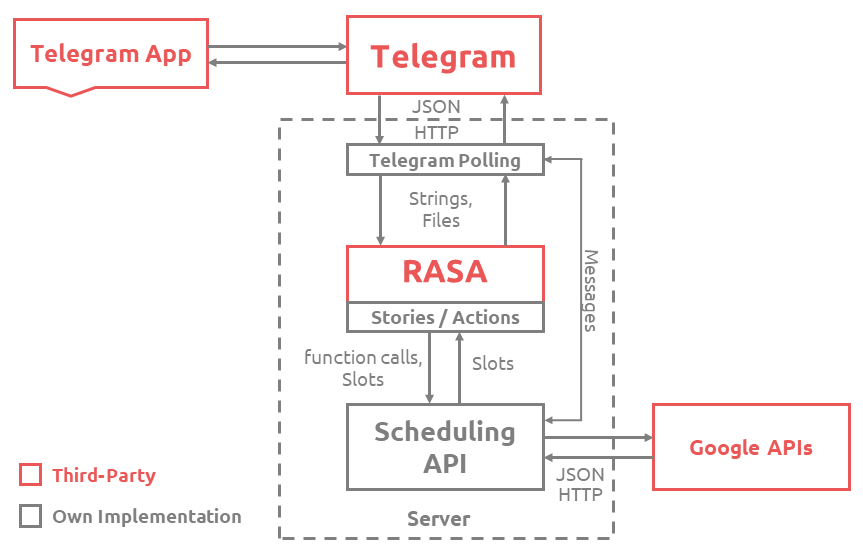
\includegraphics[width=\linewidth]{components}
\\

Für die Realisierung unseres Chatbots haben wir folgende Kernkomponenten identifiziert:

\begin{center}
	\begin{tabular}{c|l}
		\textbf{Komponente} & \makecell[c]{\textbf{Beschreibung}} \\\hline
		Telegram-Manager & \makecell[l]{Ein selbstgeschriebenes Python Modul für den Verbindungsaufbau\\zur Telegram-Schnittstelle. Benutzt u.a. die HTTP-Polling API.} \\\hline
		Planner & \makecell[l]{Selbstgeschrieben. Hauptkomponente des Terminplanens und\\-verwaltens.} \\\hline
		PlannerToImage & \makecell[l]{Selbstgeschrieben. Generiert aus einem Planner-Object eine\\PNG-Datei, die zu einer angegebenen Woche, eine visuelle\\Darstellung des Zeitplans darstellt.} \\\hline
		\makecell[c]{RASA\\Core \& NLU} & \makecell[l]{Nutzung des RASA-Frameworks der Sprachverarbeitung und\\Antwortgenerierung.}\\\hline
		\makecell[c]{RASA\\Custom-Actions} & \makecell[l]{Selbstgeschrieben. Benötigt für die Verarbeitung komplexerer\\Anfragen, bspw. Eintragen eines Termines, Anzeigen des Planes, etc.}\\\hline
		\makecell[c]{Google\\Distance-Matrix-API} & \makecell[l]{Third Patry. Genutzt für die zeitliche Distanzberechnung\\verschiedener Locations von Terminen und der daraus\\resultierenden "Route".}
	\end{tabular}
\end{center}


\section{Datenfluss und Kommunikation zwischen Komponenten}
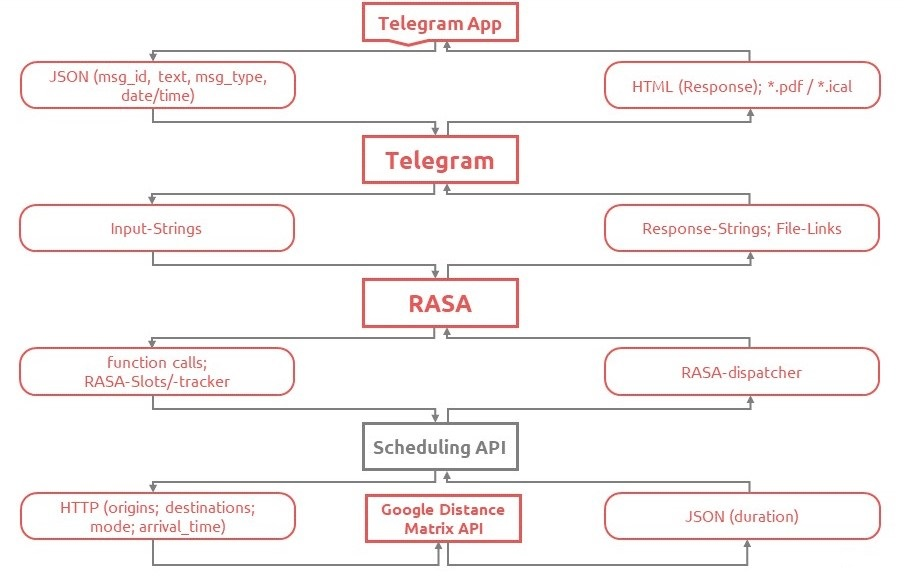
\includegraphics[width=\linewidth]{communication}\\

Zur Verdeutlichung der Kommunikationsprozesse zwischen den Komponenten folgt nun ein ideal-typischer Durchlauf durch unser System.\\

Die Telegram-API erlaubt es einem, neue Nachrichten mittels eines HTTP-Requests an den Telegram-Server abzufragen. Die genutze Strategie ist ein Long-Polling, bei dem unser Client den Request an Telegram übermittelt und erst, bei eintreffen einer neuen Nutzernachricht, eine Rückmeldung von Telegram erhält. Ist dies geschehen, überprüfen wir zunächst die Nachricht auf gesonderte Commands (bswp. "/help", "/feedback", etc.), die daraufhin ihre entsprechende Funktion ausführen. Sind diese in der Nachricht nicht enthalten, lassen wir diese durch die RASA-Pipeline analysieren. Dabei ist selbstverständlich der RASA-NLU Prozess zu erwähnen, der, entsprechend unserer vordefinierten und trainierten Story- und NLU-Daten, eine Intent-Klassifikation vornimmt. In einigen Fällen kann es passieren, dass die Ausführung einer RASA-Custom-Action notwendig wird, bspw. wenn der Nutzer ein neues Event planen möchte. Im speziellen Fall der Eventplanung nutzen wir von RASA eine Form-Action, um ein effizienteres und robusteres Setzen von Slots zu gewährleisten, als dies bei der Definition von vielen einzelnen Stories möglich wäre. Uhrzeiten, Daten und Zeitintervalle werden vom Duckling-Extractor von Facebook ermittelt. Da hierbei allerdings nur eine automatisierte Kommunikation zwischen RASA und Duckling erfolgt, auf die wir kaum Einfluss nehmen können, haben wir von weiteren Ausführungen diesbezüglich abgesehen.\\

Die Planung- und Verwaltung von Terminen und Fahrzeiten übernimmt bei uns unsere eigens geschriebene Planner-Komponente. Diese verfügt über diverse Listen von Tagen und ihren Terminen, sowie u.a. dem Planungsalgorithmus, welcher eine möglichst optimale "Route" von Terminen generiert.
Konkret wird für die Distanzberechnung der Location von Terminen die Distance-Matrix-API von Google verwendet, die je nach unseren Einstellungen eine Entfernung in Stunden und Minuten zurückgibt.\\

Wurde ein Termin erfolgreich in unserem Planner hinterlegt, so generiert RASA über unsere Story- und Templatevorlagen einen entsprechenden Antwortstring. In den meisten Fällen reichen wir diesen über unsere Telegram-Schnittstelle an den Nutzer weiter. Manchmal jedoch kann es sein, dass eine erweiterte Handlung notwendig wird, so z.B. beim zusenden unseres eigens generieten Bildes des Terminplanes. Dafür bauen wir in die Antwort der Custom-Action einen Hinweis in den String mit ein. Beim Anzeigen des Planes ist dies ein "/show\_plan" am Anfang des Strings. Diesen Teil fangen wir vorher in unserem Hauptprogramm wieder ab, und führen die Aktionen aus, die für das Bildzusenden erforderlich sind.

Schließlich, sobald alle neuen Nachrichten aller Nutzer auf diese Weise verarbeitet wurden, führen wir diese Schleife von Neuem aus, und warten mittles Polling auf die nächste Nachricht.

\section{APIs und Trainingsdatensätze}
In diesem Abschnitt nun eine kurze Übersicht, über die hauptsächlich verwendeten third-party und eigens definierten Schnittstellen, sowie externen Datensätze.

\subsection{Telegram-API}

Hauptsächlich verwenden wir für die ermittlung neuer Nutzernachrichten die öffentliche Telegram-API, wie sie unter \texttt{https://core.telegram.org/bots/api} zu finden ist. Exemplarisch zeigen wir hier ein paar unserer verwendeten Anfragen.\\

Um alle neuen Nachrichten zu erhalten, ist folgende Anfrage geeignet. Die Antwort enthält ein JSON-Objekt, untergliedert nach Nutzer-IDs, dazugehörigen Nachrichten, sowie weiteren Informationen:\\

%\begin{center}
	\texttt{
		https://api.telegram.org/bot<API-KEY>/getUpdates\\?offset=<offset>\\\&timeout=100\\\&allowed\_updates=message,callback\_query
	}\\
%\end{center}

Da Telegram alle Nachrichten intern fortlaufend indiziert, ist die Angabe eines Offset notwendig, um lediglich \textit{neue} Nachrichten zu erhalten. Der Timeout von 100 Sekunden gibt unser Intervall für das Long-Polling an. Unter Allowed-Updates ist Callback-Query für die Übermittlung von Buttons im Chatverlauf notwendig. Diese nutzen wir, um dem Nutzer eine Auswahlmöglichkeit beim Löschen von Events zu unterbreiten.\\

Zum Sender einer Nachricht zu einem Nutzer, ist folgender API-Call sinnvoll:

\texttt{https://api.telegram.org/bot<API-KEY>/sendMessage\\?chat\_id=<CHAT-ID>\\\&text=<MESSAGE>}\\

Die \texttt{chat\_id} ist eine von Telegram generierte Identifikationsnummer, die jeden Nutzer eindeutig zuordnet. Man erhält sie über den obenstehenden \texttt{getUpdates}-API Aufruf.\\

Weitere API-Requests dieser Art lassen sich in unserem Projekt finden, bspw. für das Senden und Empfangen von Bild- und anderen Dateien.


\subsection{Google Places und Distance-Matrix-API}
Wie zuvor bereits erwähnt, nutzen wir für zeitliche Distanzberechnungen die Distance-Matrix-API von Google. Für jeden API-Call berechnet Google einen Betrag, der am Monatsende zuzahlen ist. Glücklicherweise wird aberfür eine erstmalige Nutzung ein Freibetrag von 300 USD gutgeschrieben, die für unsere Tests, inklusive der Erhebung von Nutzererfahrungen, deutlich ausgereicht hat.\\
Auch in diesem Abschnitt nun eine exemplarische Listung der von uns verwendeten API-Schnittstelle:\\

Die folgende Anfrage gibt ein JSON-Object von gefunden Adressen und ihren Distanzen zurück. Die Fortbewegungsmethode kann mittels \texttt{mode}-Parameter eingestellt werden. Die Angabe von Start- und Zieladressen erfolgt über die jeweiligen Parameter \texttt{origins} und \texttt{destinations}. Die \texttt{departure\_time} gibt den Zeitpunkt des Losfahrens im UTC-Format (Sekunden seit dem 01.01.1970) an.\\

\texttt{https://maps.googleapis.com/maps/api/distancematrix/json\\?units=metric\\\&language=en\\\&region=de\\\&key=<API-KEY>\\\&origins=<START-ADDESS>\\\&destinations=<END-ADDRESS[|END-ADDRESS|...]>\\\&mode=transit\\\&departure\_time=<UTC-TIME>}\\

Für die Validierung einer angegebenen Adresse schlagen wir die Adress ebendfalls bei Google Places wiefolgt nach:\\

\texttt{https://maps.googleapis.com/maps/api/place/findplacefromtext/json\\?key=<API-KEY>\\\&inputtype=textquery\\\&language=en\\\&fields=formatted\_address\\\&input=<USER-INPUT>}\\

Über \texttt{input} geben wir die zu prüfende Adresse an und erhalten ein JSON-Object, in dem sich u.a. eine formatierte Adresse befindent, zusätzlich Postleitzahl, Stadt und Land, selbst wenn diese in der ursprünglichen Eingabe nicht vorkamen.\\
Sollte eine Adresse nicht gefunden werden, so werten wir dies als Fehler bei der Nutzereingabe oder Entity-Erkennung, und können somit bswp. zu einer erneuten Eingabe auffordern.

\subsection{Planner und PlannerToImage}
Um die Termine eines Nutzers zu planen und effiziente Zeitpläne zu erstellen, haben wir ein eigenes Planner-Modul erstellt. Dieses ist hierachisch gegliedert. Ein Planner-Object verfügt über eine List von Day-Objects, welche jeweils einen zuplanenden Tag darstellen. Jedes Day-Object wiederum hält eine Liste von eingeplanten Event-Objects, die eine vom Nutzer geplante Veranstaltung, d.h. Ort, Zeit / Dauer und Datum, repräsentiert. Ein Neuplanen von Events eines Planner-Objects erfolgt über den Methodenaufruf \texttt{Planner.replan()} und das Hinzufügen eines Events über die Methode \texttt{Planner.add\_event([...])}. Als Parameter wird ein Event-Object und, bei einem spezifischen Event, ein Datum in Form eines Arrays \texttt{[Tag, Monat, Jahr]}, übergeben. Über viele weitere Methoden der Planner-Klasse, kann die Eventplanung an die unterschiedlichen Voraussetzungen der Nutzer angepasst werden.\\
So bswp. \texttt{Planner.set\_home([...])} zum Setzen des Zuhauses eines Nutzers,\\\texttt{Planner.set\_planning\_times([...])} um die Planungsstart- und enduhrzeit zu setzen, \texttt{Planner.import\_ics([...])} und \texttt{Planner.export\_ics{[...]}} zum Im- und Exportieren von *.ical oder *.ics Dateien, u.v.m.\\

Auch die generierte Bilddatei eines Planes haben wir selber, über das Modul\\ \texttt{PlannerToImage}, erstellen müssen. Unter der Nutzung der \textit{PIL - Python Image Library} zeichnen wir daher zunächst den Hintergrund des Planerbildes und iterieren über die Tage und Events des darzustellenden Planner-Objects. Der Einfachheit halber, beschränken wir uns dabei lediglich auf die aktuelle Woche.


\subsection{Chatito und Open Addresses}
Während unserer Erfahrung mit RASA und der damit zur verfügungstehenden Entity-Extraction, haben wir festgestellt, dass eine Erkennung von Adressen in Nutzereingaben sehr schwer zu bewerkstelligen ist. Um dieses Problem anzugehen, haben wir uns mit der Generierung von großen ($>$ 1.000) Trainingsdatensätzen beschäftigt. Ein nütliches Tool, das eine eben jene zufällige Erstellung von Beispieleingaben erbringt, ist \textit{Chatito}, zu finden unter \texttt{https://github.com/rodrigopivi/Chatito}.\\

Um nun noch Chatito mit Adress-Daten zu füttern, haben wir uns für das Open-Data Projekt \textit{Open Addresses} entschieden. Der Datensatz für deutsche Adressen enthält zum derzeitigen Stand 6.271.635 unterschiedliche Adressen aus ganz Deutschland. Da wir unser RASA-Modell mit nur einem Bruchteil davon trainieren (1.000 bis 10.000 Beispiele), haben wir damit mehr als genug abgedeckt.
